\documentclass[12pt,a4paper]{article}
\usepackage[utf8]{inputenc}
\usepackage{geometry}
\geometry{a4paper, margin=1in}
\usepackage{graphicx}
\usepackage{hyperref}
\usepackage{listings}
\usepackage{color}
\usepackage{booktabs}
\usepackage{tabularx}
\usepackage{longtable}
\usepackage{float}
\usepackage{enumitem}

% Code snippet formatting
\definecolor{codegray}{rgb}{0.5,0.5,0.5}
\definecolor{codepurple}{rgb}{0.58,0,0.82}
\definecolor{backcolour}{rgb}{0.95,0.95,0.92}
\lstdefinestyle{mystyle}{
    backgroundcolor=\color{backcolour},   
    commentstyle=\color{codegray},
    keywordstyle=\color{blue},
    numberstyle=\tiny\color{codegray},
    stringstyle=\color{codepurple},
    basicstyle=\ttfamily\footnotesize,
    breakatwhitespace=false,         
    breaklines=true,                 
    captionpos=b,                    
    keepspaces=true,                 
    numbers=left,                    
    numbersep=5pt,                  
    showspaces=false,                
    showstringspaces=false,
    showtabs=false,                  
    tabsize=2
}
\lstset{style=mystyle}

% Custom title page colors
\definecolor{TitleBlue}{RGB}{0, 51, 102}

\title{} \author{} \date{} % suppress defaults

\begin{document}

% \begin{titlepage}
%     \centering
%     \vspace*{1cm}

%     % University Logo
%     
\includegraphics[width=3.5cm]{logo.png}

%     \vspace{0.8cm}

%     % University / Department
%     {\Large \textbf{Department of Computer Science \& Engineering}}\\[0.15cm]
%     {\large Independent University, Bangladesh}

%     \vspace{1.2cm}

%     % Course Header
%     {\Large \textbf{CSE-4508: RDBMS Programming Lab}}

%     \vspace{0.6cm}
%     {\color{TitleBlue}\hrule height 1.5pt}
%     \vspace{0.4cm}

%     % Project Title
%     {\huge \textbf{Project Report}}

%     \vspace{0.1cm}
%     {\LARGE \textbf{Vortex Gym Management System}}

%     \vspace{0.4cm}
%     {\color{TitleBlue}\hrule height 1.5pt}

%     \vspace{1.5cm}

%     % Team Members Table
%     {\large \textbf{Submitted By}}\\[0.4cm]
%     \begin{tabular}{l l}
%         \textbf{Abdullah Al Fahad Diganta} & 220041210 \\[0.2cm]
%         \textbf{Saom Bin Khaled}           & 220041224 \\[0.2cm]
%         \textbf{Md. Sazidur Rahman}        & 220041226 \\
%     \end{tabular}

%     \vfill

%     % Date
%     {\large \today}

% \end{titlepage}

\begin{titlepage}
    \centering
    \vspace*{0.5cm}

    % University Logo (Ensure logo.png is in the same directory)
    
\includegraphics[width=4cm]{logo.png}\\[0.5cm]

    % University / Department
    {\LARGE \textbf{Islamic University of Technology}}\\[0.2cm]
    {\Large Department of Computer Science \& Engineering}

    \vspace{1.5cm}

    % Course Header
    {\Large \textbf{Course:} CSE-4508: RDBMS Programming Lab}

    \vspace{1cm}
    {\color{TitleBlue}\hrule height 2pt}
    \vspace{0.5cm}

    % Project Title
    {\huge \textbf{Project Report}}\\[0.3cm]
    {\LARGE \textbf{Vortex Gym Management System}}

    \vspace{0.5cm}
    {\color{TitleBlue}\hrule height 2pt}

    \vspace{2cm}

    % Submission Details (Two-column layout)
    \begin{minipage}[t]{0.45\textwidth}
        \begin{flushleft}
            {\large \textbf{Submitted To:}}\\[0.2cm]
            \textbf{Sabrina Islam}\\[0.1cm]
            Lecturer\\[0.1cm]
            Department of CSE
        \end{flushleft}
    \end{minipage}
    \hfill
    \begin{minipage}[t]{0.45\textwidth}
        \begin{flushright}
            {\large \textbf{Submitted By:}}\\[0.2cm]
            \textbf{Abdullah Al Fahad Diganta} \\ ID: 220041210 \\[0.15cm]
            \textbf{Saom Bin Khaled} \\ ID: 220041224 \\[0.15cm]
            \textbf{Md. Sazidur Rahman} \\ ID: 220041226
        \end{flushright}
    \end{minipage}

    \vfill

    % Date
    % {\large \textbf{\today}}

\end{titlepage}

\tableofcontents
\newpage

\section{Problem, Scope, and Project Overview}
\subsection{Problem Statement}
Managing modern gym facilities involves handling a multitude of operations ranging from member registration, subscription billing, and class scheduling to tracking trainer availability and maintaining equipment. Many existing solutions are either fragmented across different software systems or lack the sophisticated automation needed to handle real-time validations, such as class capacity limits, overlap checking, and payment synchronization. This fragmentation leads to operational inefficiencies, billing discrepancies, double-booking classes, and a suboptimal member experience.

\subsection{Project Overview}
The \textbf{Vortex Gym Management System} is an enterprise-grade full-stack web application designed to centralize and automate gym operations. It provides a unified platform supporting four distinct user roles: Administrative, Staff, Trainer, and Member. The system seamlessly handles end-to-end gym operations including secure authentication, membership purchases, dynamic class scheduling, real-time facility access via QR codes, personnel management, and equipment tracking.

\subsection{Scope}
The scope of the project encompasses:
\begin{itemize}
    \item A web-based portal mapping out dashboards for Members, Trainers, Staff, and Admins.
    \item Integration of a real payment gateway (SSLCommerz) to handle online subscription transactions.
    \item Database-level enforcement of business rules, such as trainer shift validations and room capacity constraints using triggers and advanced queries.
    \item Analytics dashboards for business tracking, including Monthly Recurring Revenue (MRR) and usage patterns.
    \item A robust backend API using Spring Boot paired with a responsive React frontend.
\end{itemize}

\newpage
\section{List of Features}
\begin{itemize}[leftmargin=*]
    \item \textbf{Authentication \& Access Control:} Implements a secure JSON Web Token (JWT) based authentication system with robust role-based access control (RBAC). Upon login, users are routed to their respective role-specific dashboards (Admin, Staff, Trainer, or Member). It also includes a secure, token-based password reset mechanism sent via email, ensuring account recovery is safe and user-friendly.
    \item \textbf{Member Portal \& Store:} A comprehensive self-service dashboard designed for gym members. Members can seamlessly view active subscriptions, browse and purchase membership plans or class packages (monthly/yearly), and interact with a dynamic calendar to book classes. It also features profile management (including profile photo uploads) and generates a unique, dynamic QR code for automated facility check-ins.
    \item \textbf{Admin Control Panel:} The central command hub for gym management. It features detailed revenue analytics (such as Monthly Recurring Revenue and peak-time usage charts), active/inactive membership tracking, and comprehensive inventory status monitoring. Admins also oversee staff operations, review trainer applications, and monitor the Live Facility Access feed to track real-time member check-ins.
    \item \textbf{Master Schedule Builder:} A powerful scheduling engine that enables administrators to define recurring class plans (e.g., weekly Yoga or HIIT sessions). The system automatically validates against strict constraints, preventing room double-booking and ensuring trainers are not double-booked or assigned outside their working shifts.
    \item \textbf{Trainer Dashboard:} A personalized portal for fitness instructors. Trainers can view their upcoming shift schedules, check details for their assigned classes, and easily perform digital roll-calls by marking attendance for enrolled class members. The dashboard also supports waitlist visibility, helping trainers manage class capacities effectively.
    \item \textbf{Staff Portal:} Designed for front-desk and maintenance personnel, this portal provides a live view of the check-in roster, allowing staff to monitor facility entry. Additionally, it equips staff with tools to manage physical equipment inventory, such as flagging malfunctioning machines for maintenance and logging repair statuses.
    \item \textbf{Recruitment System:} A fully integrated hiring workflow featuring a public-facing careers page where prospective trainers can submit their applications and initial details. This is paired with an administrative review board that allows management to instantly approve, reject, or promote applicants directly to the Trainer role, streamlining the onboarding process.
    \item \textbf{Automated Subscriptions \& Grace Periods:} Seamless lifecycle management for memberships. The system automatically tracks subscription expiry dates, plan limits, and grace periods. This module is tightly synchronized with the SSLCommerz payment gateway via webhooks, ensuring that plans are instantly activated or updated the moment a payment succeeds, without manual intervention.
    \item \textbf{In-App Notifications \& Alerts:} A real-time notification engine that pushes system alerts directly to member dashboards based on interactions (e.g., booking confirmations, waitlist promotions). It also utilizes Spring Mail to send automated SMTP email updates for critical events like payment receipts and application status changes.
\end{itemize}

\newpage
\section{Tools and Technologies Used}
\textbf{Frontend:}
\begin{itemize}
    \item \textbf{Framework:} React (Vite environment)
    \item \textbf{Routing \& API:} React Router, Axios
    \item \textbf{Styling:} Tailwind CSS (Responsive mobile-first mapping with Dark Mode support)
\end{itemize}
\textbf{Backend:}
\begin{itemize}
    \item \textbf{Framework:} Spring Boot 3 (Java 21)
    \item \textbf{Security:} Spring Security with JWT tokens
    \item \textbf{Data Access:} Spring Data JPA / Hibernate
    \item \textbf{Integrations:} SSLCommerz Payment API, Spring Mail (SMTP)
    \item \textbf{Tools:} Maven, Spring DevTools, Lombok, MapStruct
\end{itemize}
\textbf{Database:}
\begin{itemize}
    \item \textbf{Engine:} PostgreSQL
    \item \textbf{Migration:} Flyway
\end{itemize}

\newpage
\section{Database Design}
The relational schema is meticulously designed in PostgreSQL to support a robust, enterprise-grade gym management system, comprising 17 tables that strictly adhere to normalization principles (up to the Third Normal Form, 3NF). It effectively segregates user data, scheduling operations, financial transactions, and facility assets.

\subsection{Core Design Principles and Normalization}
\begin{itemize}[leftmargin=*]
    \item \textbf{Data Integrity \& Consistency:} Foreign keys enforce strict referential integrity across all operational tables. Automated cascaded deletions (\texttt{ON DELETE CASCADE}) are cautiously applied to child records like \texttt{class\_bookings} and \texttt{trainer\_commissions} when a parent session or user is removed.
    \item \textbf{Security \& Auditing:} Security-critical data, including \texttt{password\_hash} and granular privilege roles, are stored in the core \textbf{\texttt{users}} table. Audit trail timestamps (\texttt{created\_at}, \texttt{updated\_at}) are present across major transactional tables to track historical changes.
    \item \textbf{Strategic Denormalization for Query Performance:} While highly normalized, specific columns like \texttt{current\_status} in the \texttt{users} table are intentionally denormalized. This is seamlessly maintained by a PostgreSQL trigger (\texttt{sync\_member\_status}) summarizing the \texttt{subscriptions} table, significantly speeding up heavily-accessed dashboard queries by eliminating repetitive nested joins.
\end{itemize}

\subsection{Key Entities and Relationships}
\begin{itemize}[leftmargin=*]
    \item \textbf{Users \& Authentication (\texttt{users, password\_reset\_tokens}):} The \texttt{users} table acts as the foundational entity, uniquely storing Members, Trainers, Admins, and Staff distinguished by a \texttt{role} enum. It links to \texttt{password\_reset\_tokens} to handle secure account recoveries in a one-to-many relationship.
    \item \textbf{Sales \& Subscriptions (\texttt{membership\_plans, subscriptions, invoices\_payments}):} \texttt{membership\_plans} acts as the master catalog holding pricing and recurring schedule formulas. A member's \texttt{subscriptions} represent an active lifecycle mapped directly to these plans. The \texttt{invoices\_payments} table serves as the definitive financial ledger, recording transaction events synchronized with the SSLCommerz gateway.
    \item \textbf{Class Operations \& Booking Engine (\texttt{class\_sessions, class\_bookings, rooms}):} The operational core where a \texttt{class\_session} unifies a \texttt{room}, a \texttt{trainer} (from \texttt{users}), and a discrete time-slot. Members generate \texttt{class\_bookings} (resolving a many-to-many relationship between users and sessions), which dynamically track ENROLLED or WAITLISTED statuses.
    \item \textbf{Workforce Management (\texttt{trainer\_shifts, trainer\_commissions, staff\_payments, check\_ins}):} \texttt{trainer\_shifts} define valid working hours for instructors mapped to weekdays. The system calculates payroll dynamically by logging physical facility presence into \texttt{check\_ins}, which subsequently feeds into the calculation of \texttt{staff\_payments} and class-based \texttt{trainer\_commissions}.
    \item \textbf{Physical Assets \& Feedback (\texttt{equipment, trainer\_reviews, notifications}):} \texttt{equipment} is structured as a standalone inventory tracking table for maintenance logs. \texttt{trainer\_reviews} allow members to rate their instructors after classes, linking directly back to the trainer's user ID. \texttt{notifications} function as a scalable messaging queue for pushing real-time alerts to specific users.
    \item \textbf{Recruitment Pipeline (\texttt{trainer\_applications}):} A purposefully decoupled table designed to hold public form data without creating clutter in the core \texttt{users} table until an admin officially approves and migrates an applicant via the dashboard.
\end{itemize}

\subsection{Diagram and Visuals}
The following Entity Relationship Diagram illustrates the interconnectivity among the 17 tables, highlighting the relationships and structure shaping the overall schema.

\begin{figure}[H]
    \centering
    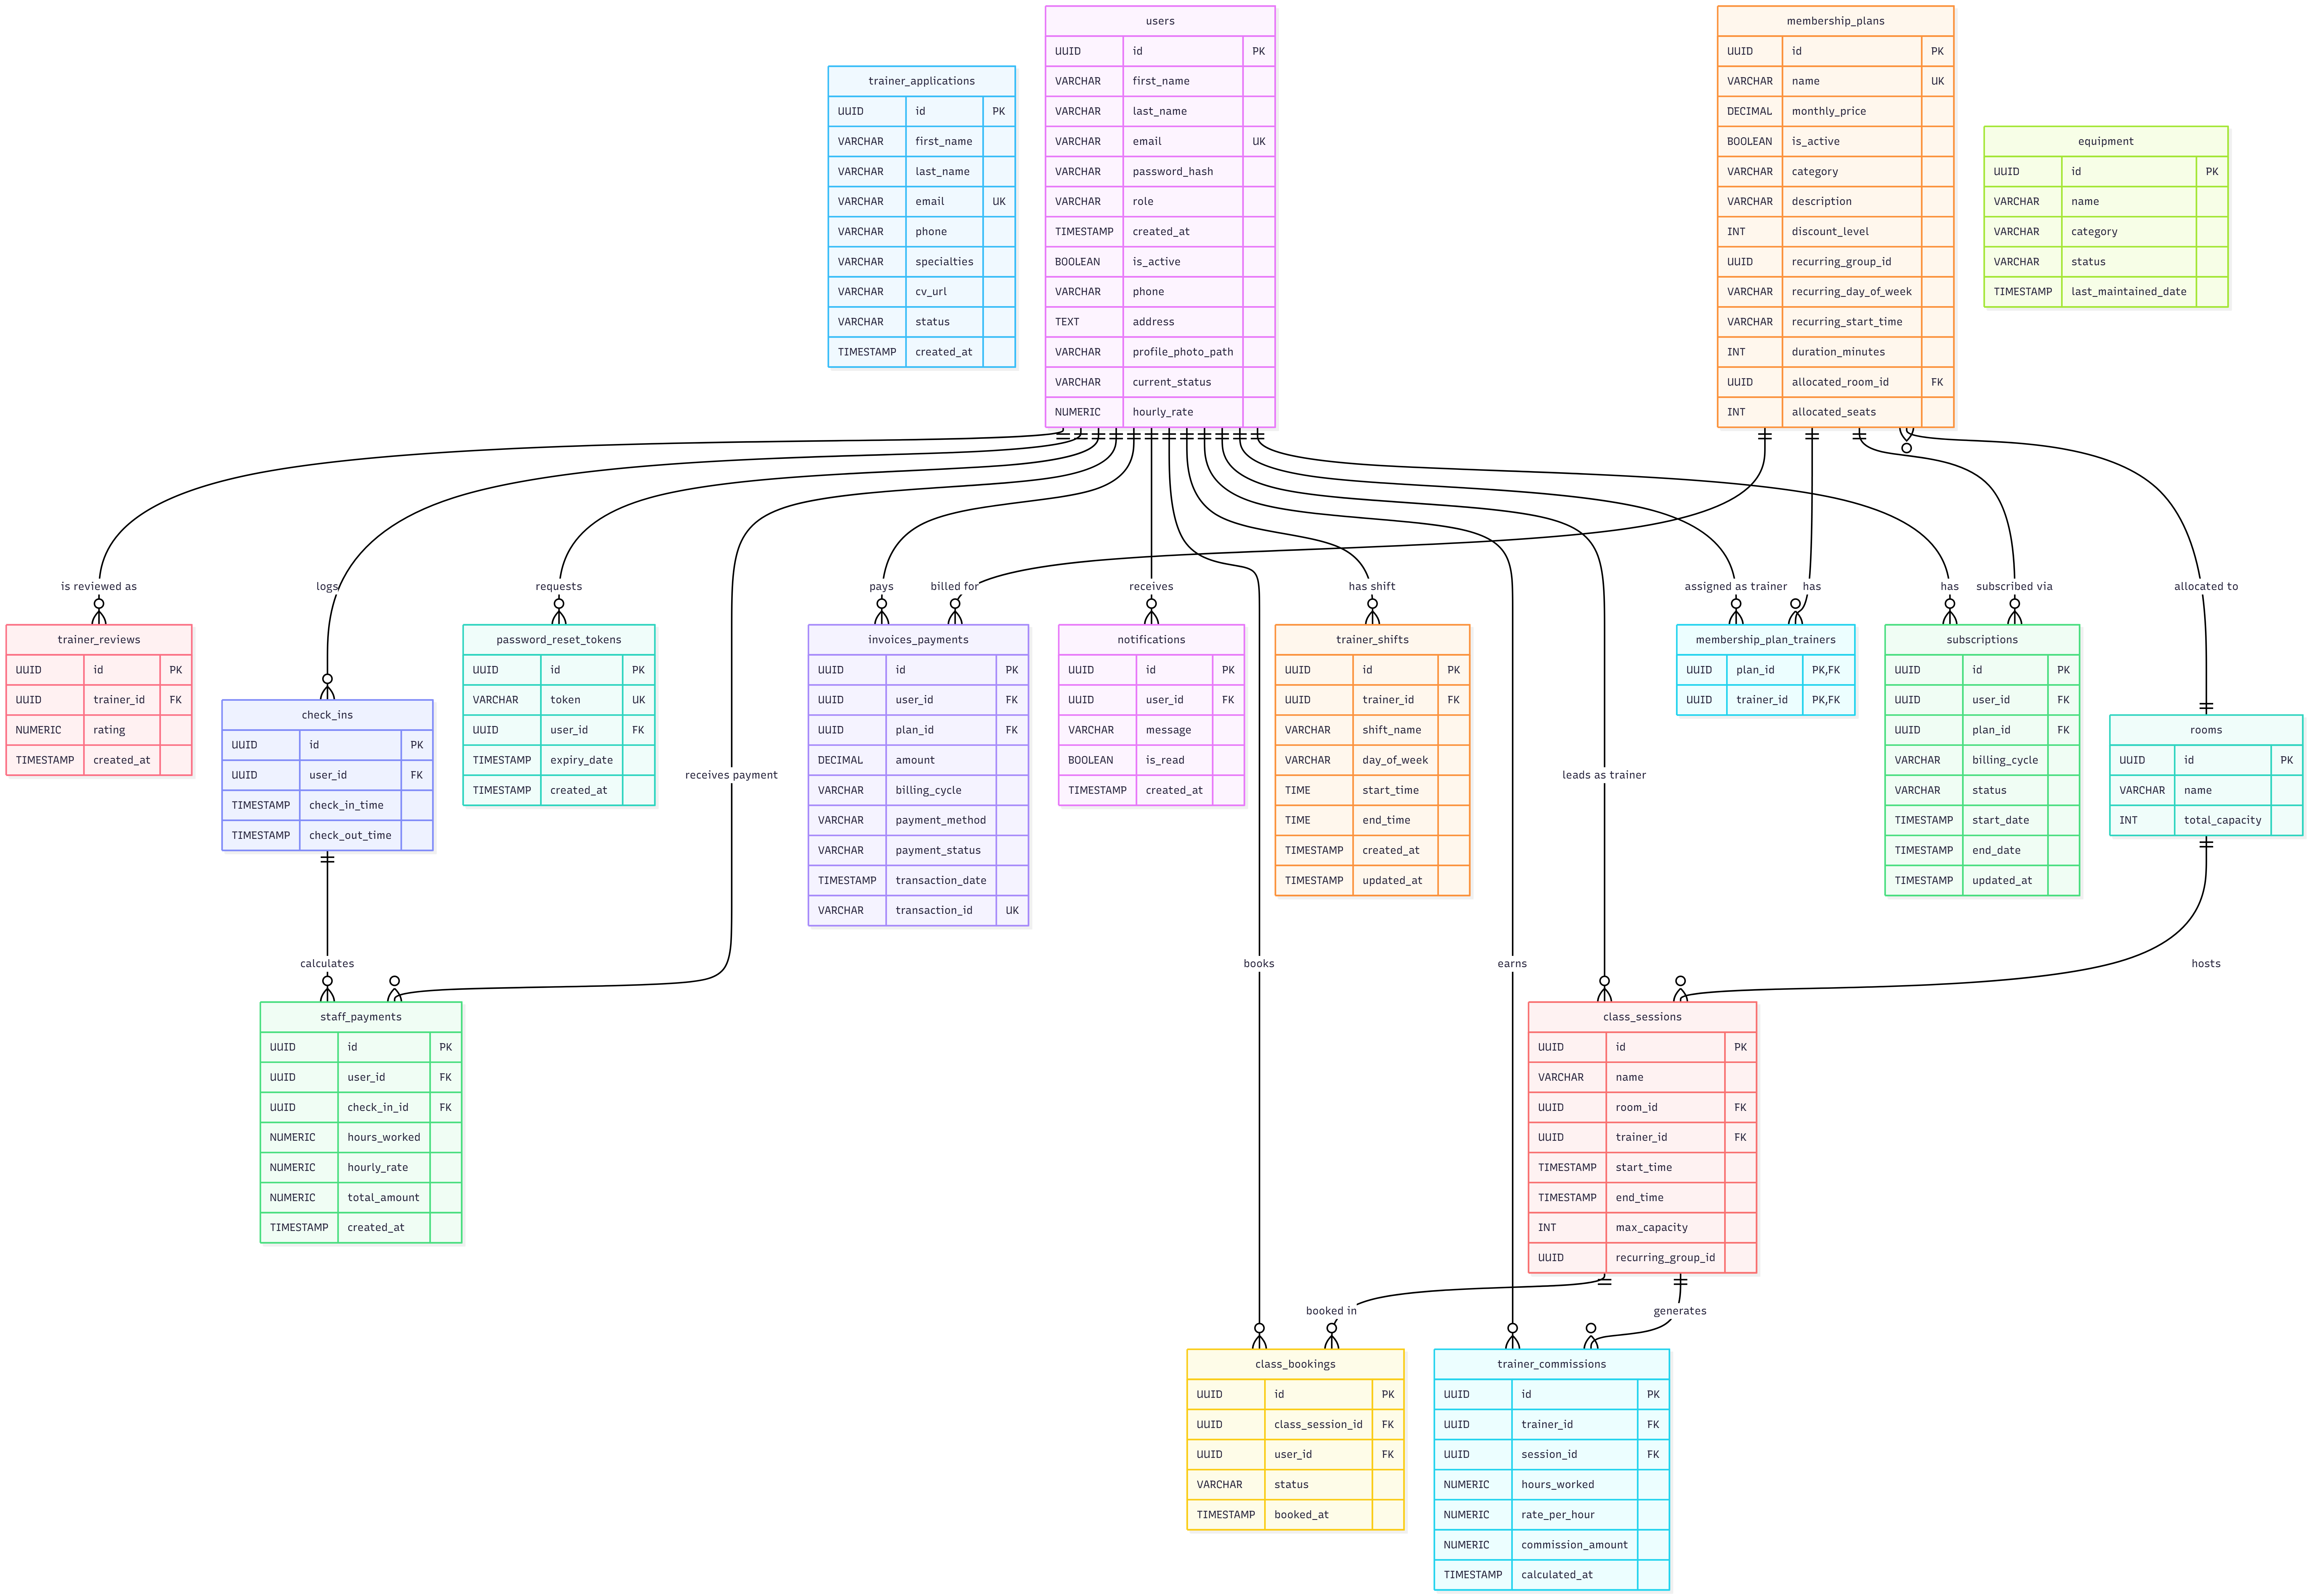
\includegraphics[width=\textwidth]{ER_D.png}
    \caption{Entity Relationship Diagram of the Vortex Gym Management System}
\end{figure}

\newpage
\section{Advanced Queries, Procedural SQL, and Concepts}

\subsection{Database Triggers}
We heavily implemented PostgreSQL triggers to enforce strict business rules directly at the database level, completely decoupled from the application service layer. This ensures data integrity even for raw SQL operations bypassing the backend.

% ---- TRIGGER 1 ----
\subsubsection*{Trigger 1: activate\_subscription\_after\_payment}
\textbf{Table:} \texttt{invoices\_payments} \quad \textbf{Event:} AFTER INSERT OR UPDATE \\
When a payment record's \texttt{payment\_status} transitions to \texttt{'SUCCESS'}, this trigger function automatically provisions or renews a row in the \texttt{subscriptions} table. It computes the correct \texttt{start\_date} and \texttt{end\_date} based on whether the billing cycle is \texttt{MONTHLY} or \texttt{YEARLY}. If an existing subscription already exists for that user-plan pair, it is updated atomically; otherwise a new one is inserted. This eliminates the need for the backend to manually handle post-payment subscription activation.

\begin{lstlisting}[language=SQL, caption=Trigger: activate\_subscription\_after\_payment]
CREATE OR REPLACE FUNCTION trg_process_successful_payment()
RETURNS TRIGGER AS $$
DECLARE
    new_end_date TIMESTAMP WITH TIME ZONE;
    existing_sub_id UUID;
BEGIN
    IF NEW.payment_status = 'SUCCESS' AND
       (TG_OP = 'INSERT' OR OLD.payment_status <> 'SUCCESS') THEN
        IF NEW.billing_cycle = 'YEARLY' THEN
            new_end_date := CURRENT_TIMESTAMP + INTERVAL '1 year';
        ELSE
            new_end_date := CURRENT_TIMESTAMP + INTERVAL '1 month';
        END IF;
        SELECT id INTO existing_sub_id FROM subscriptions
        WHERE user_id = NEW.user_id AND plan_id = NEW.plan_id LIMIT 1;
        IF existing_sub_id IS NOT NULL THEN
            UPDATE subscriptions SET
                billing_cycle = NEW.billing_cycle, status = 'ACTIVE',
                start_date = CURRENT_TIMESTAMP, end_date = new_end_date,
                updated_at = CURRENT_TIMESTAMP
            WHERE id = existing_sub_id;
        ELSE
            INSERT INTO subscriptions
                (user_id, plan_id, billing_cycle, status, start_date, end_date)
            VALUES (NEW.user_id, NEW.plan_id, NEW.billing_cycle,
                    'ACTIVE', CURRENT_TIMESTAMP, new_end_date);
        END IF;
    END IF;
    RETURN NEW;
END;
$$ LANGUAGE plpgsql;

CREATE TRIGGER activate_subscription_after_payment
AFTER INSERT OR UPDATE ON invoices_payments
FOR EACH ROW EXECUTE FUNCTION trg_process_successful_payment();
\end{lstlisting}

% ---- TRIGGER 2 ----
\subsubsection*{Trigger 2: trg\_enforce\_class\_capacity}
\textbf{Table:} \texttt{class\_bookings} \quad \textbf{Event:} BEFORE INSERT OR UPDATE \\
Before a booking row is committed, this trigger queries the current count of \texttt{'ENROLLED'} bookings for the same session. If the count equals or exceeds the session's \texttt{max\_capacity}, the incoming booking status is silently overwritten from \texttt{'ENROLLED'} to \texttt{'WAITLISTED'}, preventing overbooking entirely at the data layer.

\begin{lstlisting}[language=SQL, caption=Trigger: trg\_enforce\_class\_capacity]
CREATE OR REPLACE FUNCTION check_class_capacity()
RETURNS TRIGGER AS $$
DECLARE
    current_enrolled INT;
    class_max INT;
BEGIN
    IF NEW.status = 'ENROLLED' THEN
        SELECT COUNT(*) INTO current_enrolled FROM class_bookings
        WHERE class_session_id = NEW.class_session_id AND status = 'ENROLLED';
        SELECT max_capacity INTO class_max
        FROM class_sessions WHERE id = NEW.class_session_id;
        IF current_enrolled >= class_max THEN
            NEW.status := 'WAITLISTED';
        END IF;
    END IF;
    RETURN NEW;
END;
$$ LANGUAGE plpgsql;

CREATE TRIGGER trg_enforce_class_capacity
BEFORE INSERT OR UPDATE ON class_bookings
FOR EACH ROW EXECUTE FUNCTION check_class_capacity();
\end{lstlisting}

% ---- TRIGGER 3 ----
\subsubsection*{Trigger 3: validate\_trainer\_shift}
\textbf{Table:} \texttt{class\_sessions} \quad \textbf{Event:} BEFORE INSERT \\
Prevents scheduling a class outside the assigned trainer's registered working hours. It extracts the weekday and time from the session's \texttt{start\_time}, then queries the \texttt{trainer\_shifts} table for a valid overlapping shift. If no valid shift is found, a hard \texttt{RAISE EXCEPTION} blocks the insertion, ensuring all class sessions are always within sanctioned trainer availability.

\begin{lstlisting}[language=SQL, caption=Trigger: validate\_trainer\_shift]
CREATE OR REPLACE FUNCTION validate_trainer_shift()
RETURNS TRIGGER AS $$
DECLARE
    shift_exists BOOLEAN;
    day_name VARCHAR(20);
    class_start_time TIME;
    class_end_time TIME;
BEGIN
    day_name := CASE TO_CHAR(NEW.start_time, 'D')::INT
        WHEN 1 THEN 'SUNDAY'   WHEN 2 THEN 'MONDAY'
        WHEN 3 THEN 'TUESDAY'  WHEN 4 THEN 'WEDNESDAY'
        WHEN 5 THEN 'THURSDAY' WHEN 6 THEN 'FRIDAY'
        WHEN 7 THEN 'SATURDAY'
    END;
    class_start_time := NEW.start_time::TIME;
    class_end_time   := NEW.end_time::TIME;
    SELECT EXISTS(
        SELECT 1 FROM trainer_shifts
        WHERE trainer_id = NEW.trainer_id
          AND day_of_week = day_name
          AND start_time <= class_start_time
          AND end_time   >= class_end_time
    ) INTO shift_exists;
    IF NOT shift_exists THEN
        RAISE EXCEPTION
            'Class scheduled outside trainer shift. Trainer: %, Day: %',
            NEW.trainer_id, day_name;
    END IF;
    RETURN NEW;
END;
$$ LANGUAGE plpgsql;

CREATE TRIGGER validate_trainer_shift
BEFORE INSERT ON class_sessions
FOR EACH ROW EXECUTE FUNCTION validate_trainer_shift();
\end{lstlisting}

% ---- TRIGGER 4 ----
\subsubsection*{Trigger 4: sync\_member\_status}
\textbf{Table:} \texttt{subscriptions} \quad \textbf{Event:} AFTER INSERT OR UPDATE \\
This trigger implements \textbf{strategic denormalization}. Whenever a subscription's status changes, it immediately reflects the new status into the \texttt{current\_status} column on the \texttt{users} table. This avoids a repeated expensive JOIN to \texttt{subscriptions} on every member dashboard API call, providing a real-time, pre-aggregated status flag at the user record level.

\begin{lstlisting}[language=SQL, caption=Trigger: sync\_member\_status]
CREATE OR REPLACE FUNCTION sync_member_status()
RETURNS TRIGGER AS $$
DECLARE
    member_status VARCHAR(20);
BEGIN
    SELECT status INTO member_status FROM subscriptions
    WHERE user_id = NEW.user_id ORDER BY updated_at DESC LIMIT 1;
    member_status := COALESCE(member_status, 'INACTIVE');
    UPDATE users SET current_status = member_status WHERE id = NEW.user_id;
    RETURN NEW;
END;
$$ LANGUAGE plpgsql;

CREATE TRIGGER sync_member_status
AFTER INSERT OR UPDATE ON subscriptions
FOR EACH ROW EXECUTE FUNCTION sync_member_status();
\end{lstlisting}

\subsection{Stored PL/pgSQL Functions}

% ---- FUNCTION 1 ----
\subsubsection*{Function 1: book\_class\_slot}
\textbf{Returns:} JSON \\
An atomic, multi-validation booking procedure. It sequentially executes: (1) a \textbf{duplicate booking guard}, (2) a \textbf{time-overlap conflict check} against all other sessions the member is enrolled in, and (3) a \textbf{capacity pre-check} to determine \texttt{ENROLLED} vs \texttt{WAITLISTED} status before writing to \texttt{class\_bookings}. The result is a structured JSON response, enabling clean API integration.

\begin{lstlisting}[language=SQL, caption=Function: book\_class\_slot]
CREATE OR REPLACE FUNCTION book_class_slot(p_user_id UUID, p_session_id UUID)
RETURNS JSON AS $$
DECLARE
    v_conflict_count   INT;   v_current_enrolled INT;   v_class_max INT;
    v_booking_status   VARCHAR(20);   v_new_booking_id UUID;
    v_session_start    TIMESTAMP WITH TIME ZONE;
    v_session_end      TIMESTAMP WITH TIME ZONE;
BEGIN
    -- 1. Duplicate Guard
    IF EXISTS (SELECT 1 FROM class_bookings
               WHERE class_session_id = p_session_id AND user_id = p_user_id)
    THEN RETURN json_build_object('success',false,'error','Already booked.');
    END IF;
    -- 2. Load session window
    SELECT start_time, end_time INTO v_session_start, v_session_end
    FROM class_sessions WHERE id = p_session_id;
    -- 3. Schedule Overlap Check
    SELECT COUNT(*) INTO v_conflict_count
    FROM class_bookings cb JOIN class_sessions cs ON cb.class_session_id = cs.id
    WHERE cb.user_id = p_user_id
      AND cb.status IN ('ENROLLED','WAITLISTED')
      AND cs.id != p_session_id
      AND cs.start_time < v_session_end
      AND cs.end_time   > v_session_start;
    IF v_conflict_count > 0 THEN
        RETURN json_build_object('success',false,'error','Time conflict.');
    END IF;
    -- 4. Capacity Resolution
    SELECT COUNT(*) INTO v_current_enrolled FROM class_bookings
    WHERE class_session_id = p_session_id AND status = 'ENROLLED';
    SELECT max_capacity INTO v_class_max FROM class_sessions WHERE id=p_session_id;
    v_booking_status := CASE WHEN v_current_enrolled >= v_class_max
                             THEN 'WAITLISTED' ELSE 'ENROLLED' END;
    -- 5. Atomic Insert (capacity trigger re-validates independently)
    INSERT INTO class_bookings (class_session_id, user_id, status)
    VALUES (p_session_id, p_user_id, v_booking_status)
    RETURNING id, status INTO v_new_booking_id, v_booking_status;
    RETURN json_build_object('success',true,'bookingId',v_new_booking_id,
                             'status',v_booking_status);
EXCEPTION WHEN OTHERS THEN
    RETURN json_build_object('success',false,'error',SQLERRM);
END;
$$ LANGUAGE plpgsql;
\end{lstlisting}

% ---- FUNCTION 2 ----
\subsubsection*{Function 2: assign\_trainer (with UPSERT)}
\textbf{Returns:} JSON \\
Reassigns a trainer to a session and atomically upserts a commission record. Uses \texttt{EXTRACT EPOCH} to convert session duration to hours, computes commission, and then employs \texttt{ON CONFLICT (session\_id) DO UPDATE} to guarantee a single commission row per session — a safer atomic merge versus a separate SELECT-then-INSERT.

\begin{lstlisting}[language=SQL, caption=Function: assign\_trainer with ON CONFLICT UPSERT]
CREATE OR REPLACE FUNCTION assign_trainer(
    p_session_id UUID, p_trainer_id UUID, p_rate_per_hour NUMERIC DEFAULT 15.00)
RETURNS JSON AS $$
DECLARE
    v_hours_worked      NUMERIC;
    v_commission_amount NUMERIC;
BEGIN
    IF NOT EXISTS (SELECT 1 FROM users WHERE id = p_trainer_id
                   AND role = 'TRAINER' AND is_active = TRUE) THEN
        RETURN json_build_object('success',false,'error','Trainer not found.');
    END IF;
    SELECT EXTRACT(EPOCH FROM (end_time - start_time)) / 3600.0
    INTO v_hours_worked FROM class_sessions WHERE id = p_session_id;
    v_commission_amount := ROUND(v_hours_worked * p_rate_per_hour, 2);
    UPDATE class_sessions SET trainer_id = p_trainer_id WHERE id = p_session_id;
    -- UPSERT: one commission record per session (UNIQUE on session_id)
    INSERT INTO trainer_commissions
        (trainer_id, session_id, hours_worked, rate_per_hour, commission_amount)
    VALUES (p_trainer_id, p_session_id, v_hours_worked,
            p_rate_per_hour, v_commission_amount)
    ON CONFLICT (session_id) DO UPDATE SET
        trainer_id        = EXCLUDED.trainer_id,
        hours_worked      = EXCLUDED.hours_worked,
        commission_amount = EXCLUDED.commission_amount,
        calculated_at     = CURRENT_TIMESTAMP;
    RETURN json_build_object('success',true,'commissionAmount',v_commission_amount);
EXCEPTION WHEN OTHERS THEN
    RETURN json_build_object('success',false,'error',SQLERRM);
END;
$$ LANGUAGE plpgsql;
\end{lstlisting}

% ---- FUNCTION 3 ----
\subsubsection*{Function 3: get\_used\_capacity\_for\_room\_at\_time}
\textbf{Returns:} INTEGER \\
Sums the \texttt{max\_capacity} of all class sessions that overlap with a proposed time window in a given room. Used during schedule creation to prevent exceeding a room's physical spatial limits with multiple overlapping sessions.

\begin{lstlisting}[language=SQL, caption=Function: get\_used\_capacity\_for\_room\_at\_time]
CREATE OR REPLACE FUNCTION get_used_capacity_for_room_at_time(
    p_room_id UUID, p_start_time TIMESTAMPTZ, p_end_time TIMESTAMPTZ)
RETURNS INTEGER AS $$
DECLARE v_used_capacity INTEGER;
BEGIN
    SELECT COALESCE(SUM(cs.max_capacity), 0) INTO v_used_capacity
    FROM class_sessions cs
    WHERE cs.room_id = p_room_id
      AND cs.start_time < p_end_time
      AND cs.end_time   > p_start_time;
    RETURN v_used_capacity;
END;
$$ LANGUAGE plpgsql STABLE;
\end{lstlisting}

% ---- FUNCTION 4 ----
\subsubsection*{Function 4: count\_overlapping\_trainer\_classes}
\textbf{Returns:} BIGINT \\
Counts how many sessions a trainer already has that overlap with a new proposed time slot. An optional \texttt{p\_exclude\_session\_id} parameter avoids self-conflict when editing an existing session. Called as a pre-validation guard before every scheduling write to enforce trainer exclusivity.

\begin{lstlisting}[language=SQL, caption=Function: count\_overlapping\_trainer\_classes]
CREATE OR REPLACE FUNCTION count_overlapping_trainer_classes(
    p_trainer_id UUID, p_start_time TIMESTAMPTZ, p_end_time TIMESTAMPTZ,
    p_exclude_session_id UUID DEFAULT NULL)
RETURNS BIGINT AS $$
DECLARE v_overlap_count BIGINT;
BEGIN
    SELECT COUNT(*) INTO v_overlap_count FROM class_sessions cs
    WHERE cs.trainer_id = p_trainer_id
      AND cs.start_time < p_end_time
      AND cs.end_time   > p_start_time
      AND (p_exclude_session_id IS NULL OR cs.id <> p_exclude_session_id);
    RETURN v_overlap_count;
END;
$$ LANGUAGE plpgsql STABLE;
\end{lstlisting}

% ---- FUNCTION 5 ----
\subsubsection*{Function 5: get\_member\_available\_classes}
\textbf{Returns:} TABLE \\
Returns all future class sessions that fall within a member's active subscription date window, joining room and trainer data for a complete calendar payload. A subscription-gate is enforced at the database level: members without an \texttt{ACTIVE} subscription see zero rows, requiring no application-side filtering.

\begin{lstlisting}[language=SQL, caption=Function: get\_member\_available\_classes]
CREATE OR REPLACE FUNCTION get_member_available_classes(p_user_id UUID)
RETURNS TABLE (session_id UUID, name VARCHAR, start_time TIMESTAMPTZ,
               end_time TIMESTAMPTZ, max_capacity INT, room_id UUID,
               room_name VARCHAR, trainer_id UUID, trainer_first_name VARCHAR,
               trainer_last_name VARCHAR, remaining_capacity BIGINT) AS $$
BEGIN
    RETURN QUERY
    SELECT cs.id, cs.name, cs.start_time, cs.end_time, cs.max_capacity,
           rm.id, rm.name, tr.id, tr.first_name, tr.last_name,
           cs.max_capacity::BIGINT
    FROM class_sessions cs
    JOIN rooms rm ON rm.id = cs.room_id
    JOIN users tr ON tr.id = cs.trainer_id
    WHERE cs.start_time > CURRENT_TIMESTAMP
      AND EXISTS (
          SELECT 1 FROM subscriptions s
          WHERE s.user_id = p_user_id AND s.status = 'ACTIVE'
            AND cs.start_time BETWEEN
                COALESCE(s.start_date, CURRENT_TIMESTAMP - INTERVAL '1 day')
                AND COALESCE(s.end_date, CURRENT_TIMESTAMP + INTERVAL '5 years'))
    ORDER BY cs.start_time ASC;
END;
$$ LANGUAGE plpgsql STABLE;
\end{lstlisting}

\subsection{Advanced Analytical SQL Queries}

% ---- QUERY 1 ----
\subsubsection*{Query 1: peak\_hours\_analysis (GROUPING SETS)}
\textbf{Returns:} TABLE \\
Aggregates check-in logs using \textbf{GROUPING SETS} — a powerful SQL extension that computes multiple aggregation levels within a single query scan. It simultaneously produces counts per day-hour combination, per-day totals, per-hour totals (for the peak-hour bar chart), and an overall grand total. This avoids four separate \texttt{UNION ALL} queries.

\begin{lstlisting}[language=SQL, caption=Function: peak\_hours\_analysis using GROUPING SETS]
CREATE OR REPLACE FUNCTION peak_hours_analysis()
RETURNS TABLE (day_label TEXT, hour_label INTEGER,
               checkins_count BIGINT, grouping_level TEXT) AS $$
BEGIN
    RETURN QUERY
    SELECT
        CASE WHEN GROUPING(day_name)=1 THEN 'ALL_DAYS' ELSE day_name END,
        CASE WHEN GROUPING(hour_val) =1 THEN NULL       ELSE hour_val  END,
        COUNT(*)::BIGINT,
        CASE
            WHEN GROUPING(day_name)=0 AND GROUPING(hour_val)=0 THEN 'DAY_HOUR'
            WHEN GROUPING(day_name)=0 AND GROUPING(hour_val)=1 THEN 'DAY_TOTAL'
            WHEN GROUPING(day_name)=1 AND GROUPING(hour_val)=0 THEN 'HOUR_TOTAL'
            ELSE 'GRAND_TOTAL'
        END
    FROM (SELECT TO_CHAR(ci.check_in_time,'Dy') AS day_name,
                 EXTRACT(HOUR FROM ci.check_in_time)::INT AS hour_val
          FROM check_ins ci) attendance
    GROUP BY GROUPING SETS ((day_name, hour_val), (day_name), (hour_val), ())
    ORDER BY CASE WHEN GROUPING(day_name)=1 THEN 1 ELSE 0 END,
             day_label, hour_label;
END;
$$ LANGUAGE plpgsql STABLE;
\end{lstlisting}

% ---- QUERY 2 ----
\subsubsection*{Query 2: top\_trainers\_ranking (CTEs + DENSE\_RANK Window Function)}
\textbf{Returns:} TABLE \\
Uses a chain of \textbf{Common Table Expressions (CTEs)} to decompose a multi-step aggregation plan, followed by the \textbf{DENSE\_RANK} window function to generate a trainer leaderboard based on class attendance retention rate. Tied trainers share the same rank position, which is semantically correct for a competitive ranking (unlike \texttt{ROW\_NUMBER}).

\begin{lstlisting}[language=SQL, caption=Function: top\_trainers\_ranking with CTEs and DENSE\_RANK]
CREATE OR REPLACE FUNCTION top_trainers_ranking()
RETURNS TABLE (trainer_id UUID, first_name VARCHAR, last_name VARCHAR,
               attended_count BIGINT, attendance_events BIGINT,
               retention_rate NUMERIC, rank_position BIGINT) AS $$
BEGIN
    RETURN QUERY
    WITH trainer_attendance AS (
        SELECT cs.trainer_id,
            SUM(CASE WHEN cb.status = 'PRESENT' THEN 1 ELSE 0 END)::BIGINT AS attended_count,
            SUM(CASE WHEN cb.status IN ('PRESENT','ABSENT') THEN 1 ELSE 0 END)::BIGINT AS attendance_events
        FROM class_sessions cs
        LEFT JOIN class_bookings cb ON cb.class_session_id = cs.id
        GROUP BY cs.trainer_id
    ),
    trainer_scores AS (
        SELECT ta.trainer_id, ta.attended_count, ta.attendance_events,
               COALESCE(ROUND((ta.attended_count * 100.0)
                              / NULLIF(ta.attendance_events, 0), 2), 0) AS retention_rate
        FROM trainer_attendance ta
    )
    SELECT u.id, u.first_name, u.last_name,
           ts.attended_count, ts.attendance_events, ts.retention_rate,
           DENSE_RANK() OVER (ORDER BY ts.retention_rate DESC,
                                       ts.attendance_events DESC)
    FROM trainer_scores ts
    JOIN users u ON u.id = ts.trainer_id
    WHERE u.role = 'TRAINER'
    ORDER BY rank_position, u.first_name, u.last_name;
END;
$$ LANGUAGE plpgsql STABLE;
\end{lstlisting}

% ---- QUERY 3 ----
\subsubsection*{Query 3: monthly\_revenue\_rollup (ROLLUP)}
\textbf{Returns:} TABLE \\
Uses the \textbf{ROLLUP} operator to generate a hierarchical revenue summary — per-month-per-plan-category rows and a per-month subtotal — in a single query pass. This powers the revenue breakdown panel on the Admin Dashboard, distinguishing between \texttt{BASE\_MEMBERSHIP} and class-tier revenues automatically.

\begin{lstlisting}[language=SQL, caption=Function: monthly\_revenue\_rollup using ROLLUP]
CREATE OR REPLACE FUNCTION monthly_revenue_rollup()
RETURNS TABLE (revenue_month DATE, plan_type TEXT, total_income NUMERIC) AS $$
BEGIN
    RETURN QUERY
    SELECT
        DATE_TRUNC('month', ip.transaction_date)::DATE AS revenue_month,
        COALESCE(mp.category, 'ALL_PLAN_TYPES')::TEXT  AS plan_type,
        COALESCE(SUM(ip.amount), 0)                    AS total_income
    FROM invoices_payments ip
    JOIN membership_plans mp ON mp.id = ip.plan_id
    WHERE ip.payment_status = 'SUCCESS'
    GROUP BY DATE_TRUNC('month', ip.transaction_date), ROLLUP(mp.category)
    ORDER BY revenue_month DESC, plan_type;
END;
$$ LANGUAGE plpgsql STABLE;
\end{lstlisting}

% ---- QUERY 4 ----
\subsubsection*{Query 4: debtor\_list\_active (Correlated CTEs)}
\textbf{Returns:} TABLE \\
Surfaces members who are physically inside the facility (open check-in: \texttt{check\_out\_time IS NULL}) while also having overdue invoices. Uses two independent CTEs — one for active check-ins and one for overdue payments — joined against the \texttt{users} table. A practical operational query for front-desk staff alerting.

\begin{lstlisting}[language=SQL, caption=Function: debtor\_list\_active using Correlated CTEs]
CREATE OR REPLACE FUNCTION debtor_list_active()
RETURNS TABLE (user_id UUID, first_name VARCHAR, last_name VARCHAR, email VARCHAR,
               latest_check_in TIMESTAMPTZ, overdue_invoices BIGINT,
               overdue_amount NUMERIC) AS $$
BEGIN
    RETURN QUERY
    WITH active_checkins AS (
        SELECT ci.user_id, MAX(ci.check_in_time) AS latest_check_in
        FROM check_ins ci WHERE ci.check_out_time IS NULL
        GROUP BY ci.user_id
    ),
    overdue AS (
        SELECT ip.user_id,
               COUNT(*)::BIGINT    AS overdue_invoices,
               COALESCE(SUM(ip.amount), 0) AS overdue_amount
        FROM invoices_payments ip WHERE ip.payment_status = 'OVERDUE'
        GROUP BY ip.user_id
    )
    SELECT u.id, u.first_name, u.last_name, u.email,
           ac.latest_check_in, od.overdue_invoices, od.overdue_amount
    FROM active_checkins ac
    JOIN overdue od ON od.user_id = ac.user_id
    JOIN users u    ON u.id       = ac.user_id
    ORDER BY ac.latest_check_in DESC;
END;
$$ LANGUAGE plpgsql STABLE;
\end{lstlisting}

\subsection{Advanced Concepts Summary}

\begin{itemize}[leftmargin=*]
    \item \textbf{Strategic Denormalization + Trigger Sync:} The \texttt{users.current\_status} column caches each member's latest subscription state, maintained automatically by the \texttt{sync\_member\_status} trigger. This eliminates the need to JOIN \texttt{subscriptions} on every member dashboard request, trading a minimal write overhead for significant read-path performance.

    \item \textbf{UPSERT with ON CONFLICT:} The \texttt{assign\_trainer} function uses \texttt{INSERT ... ON CONFLICT (session\_id) DO UPDATE} to atomically merge commission records. This eliminates race conditions present in a naive SELECT-then-INSERT pattern and ensures exactly one commission row per session.

    \item \textbf{GROUPING SETS \& ROLLUP:} Used in \texttt{peak\_hours\_analysis()} and \texttt{monthly\_revenue\_rollup()} respectively. These constructs compute multiple GROUP BY hierarchies in one query pass, avoiding the performance cost and redundancy of chained \texttt{UNION ALL} statements.

    \item \textbf{Window Functions (DENSE\_RANK):} Applied in \texttt{top\_trainers\_ranking()} to generate a shared-rank competitive leaderboard based on trainer retention rate. Produces semantically correct results for ties, unlike \texttt{ROW\_NUMBER}.

    \item \textbf{Common Table Expressions (CTEs):} Used across multiple analytical functions to decompose complex multi-step aggregations into named, readable \texttt{WITH} blocks. CTEs improve maintainability, are often materialized by the planner for intermediate result reuse, and keep function bodies clean.

    \item \textbf{Composite Indexing for Query Optimization:} Targeted multi-column indexes were created to match the query planner's access patterns. Key examples: \texttt{idx\_class\_sessions\_room\_time (room\_id, start\_time, end\_time)} for room overlap checks, and \texttt{idx\_subscriptions\_user\_status\_window} for member calendar lookups, dramatically reducing full-table scans.

    \item \textbf{Schema Versioning via Flyway:} All DDL changes, trigger/function definitions, and seed data are managed through sequentially numbered Flyway migration files (\texttt{V1} through \texttt{V13}), providing a deterministic, auditable, and reproducible database history critical for team collaboration and CI/CD deployments.
\end{itemize}


\newpage
\section{Limitations of the Project}
The following limitations were identified as deliberate scoping decisions made to keep the project focused on core RDBMS concepts and deliverable within the semester timeline.
\begin{itemize}[leftmargin=*]
    \item \textbf{Single-Location Architecture:} The database schema is intentionally designed around a single physical gym facility. Supporting a multi-branch franchise model would require introducing a \texttt{facilities} entity and refactoring nearly all foreign key relationships to be facility-scoped — a significant schema redesign that was outside the project's intended scope.

    % \item \textbf{No Automated Subscription Expiry:} While subscription activation is fully automated via triggers, expiry handling (marking \texttt{ACTIVE} subscriptions as \texttt{EXPIRED} after \texttt{end\_date}) is not performed by a scheduled database job (e.g., \texttt{pg\_cron}). In a production system, a periodic stored procedure or a cron-triggered function would be required to sweep and deactivate stale subscriptions.

    \item \textbf{No Table Partitioning:} High-volume tables such as \texttt{check\_ins} and \texttt{invoices\_payments} are not partitioned by date range. As data grows over months or years, query performance on these tables would degrade. PostgreSQL's native range partitioning (e.g., monthly partitions on \texttt{check\_in\_time}) would be the recommended production optimization.

    \item \textbf{Software-Based QR Check-In:} The QR code facility access system operates entirely as a software scan within the browser. A production deployment would require integration with physical IoT turnstile hardware and a dedicated embedded reader — a hardware layer outside the scope of this RDBMS-focused project.

    \item \textbf{Limited Predictive Analytics:} The dashboard provides descriptive statistics (MRR, peak hours, churn rate) computed via SQL aggregations. However, predictive capabilities such as churn forecasting or personalized class recommendations would require machine learning pipelines operating outside of PostgreSQL, which was beyond the project's database-centric focus.
\end{itemize}

\section{Modifications to Initial Scope \& Design}
Throughout the semester's development path, several modifications were made over the original scope:
\begin{itemize}
    \item \textbf{Migration of Business Logic to Database:} Initially proposed to handle room booking availability and trainer validation strictly from Spring Boot services. We migrated these rules explicitly into PostgreSQL triggers (\texttt{validate\_trainer\_shift}, \texttt{check\_class\_capacity}) ensuring data consistency even from raw SQL inserts.
    \item \textbf{Payment Systems Transition:} Originally intended to implement a mock checkout protocol. We evolved this to incorporate the \textbf{SSLCommerz} integration for true localized payment handling, pushing WebHook validations into the system.
    \item \textbf{Refined User Roles:} We split the "Management" role down into separate \textbf{Admin} and \textbf{Staff} roles. This ensures granular security so general front-desk staff can only monitor attendance/inventory, while Admins deal with recurring financial plans.
\end{itemize}

\newpage
\section{Individual Contribution}
\begin{table}[H]
    \centering
    \begin{tabular}{|l|p{10cm}|}
    \hline
    \textbf{Team Member} & \textbf{Contributions} \\
    \hline
    Abdullah Al Fahad Diganta & Developed the Admin Dashboard analytics interface — revenue charts (MRR, peak hours, churn rate), membership tracking panels, and the responsive Tailwind-based layout system across all dashboards. Built the Trainer Dashboard end-to-end (shift schedule view, class roster, attendance marking UI and API). Authored the advanced analytical queries: \texttt{peak\_hours\_analysis} (GROUPING SETS), \texttt{top\_trainers\_ranking} (CTEs + DENSE\_RANK), \texttt{monthly\_revenue\_rollup} (ROLLUP), and \texttt{debtor\_list\_active}. \\
    \hline
    Saom Bin Khaled & Implemented the JWT-based authentication system (backend security + login/register UI), SSLCommerz payment gateway integration (webhook handling + store frontend), and the Master Schedule Builder (room/trainer conflict validation logic, scheduling API, and admin scheduling UI). Built the Member Portal end-to-end — dashboard UI, subscription store, class calendar with booking flow, QR code generation, and profile photo uploads. Authored the \texttt{get\_member\_available\_classes} function, \texttt{activate\_subscription\_after\_payment} trigger, and the \texttt{validate\_trainer\_shift} trigger. \\
    \hline
    Md. Sazidur Rahman & Developed the Admin Control Panel's operational modules — trainer application review board (UI + approval/rejection API), membership plan CRUD management, and room/equipment configuration. Built the Staff Portal (live check-in roster, equipment inventory and maintenance flagging). Authored the \texttt{book\_class\_slot} stored function, \texttt{trg\_enforce\_class\_capacity} and \texttt{sync\_member\_status} triggers. Designed the Flyway migration structure and ER Diagram. Integrated the Spring Mail SMTP notification system and the public-facing careers page. \\
    \hline
    \end{tabular}
\end{table}

\section{Github Link}
The fully documented source code of Vortex Gym Management System can be accessed at: \\ \\
\url{https://github.com/greenbinjack/vortex-fitness-system}

\end{document}
